\section{Experiments and Results}

We tested LCGC model in two different experimental settings. First, we test the impact of different parameters on classification performance using  artificial dataset generated through similar procedure as in previous section. LAter, we use  synthetic control dataset [Reference]  as a benchmark dataset to compare the classification performance of our model against some fundamental classification models.
In a classification setting specially in the scenarios with huge mismatch in number of instances that belong to different categories, accuracy does not provide complete picture and hence we also report F1-Scores as the measure of model’s performance. Reconstruction errors are another important metric which when compared between training and test instances can give us an approximate overview of  over-fitting in the model and thus are reported for the first experiment set. 

\subsection{Artifical data set}

In most of the classification scenarios with multi-series data, number of dimensions in observations (number of sensors for example in sensor data) and sampling resolution (number of samples per sensor) are some important factors that impact predictive performance of models. In this expriment we use an artificial generated dataset to test LCGC's performance  with varying values of output dimension (C) and sampling resolution (N) in datset. Furthermore, we also test model's performance with different number of inducing variable to test model's scalability.
\begin{figure}
    \centering
    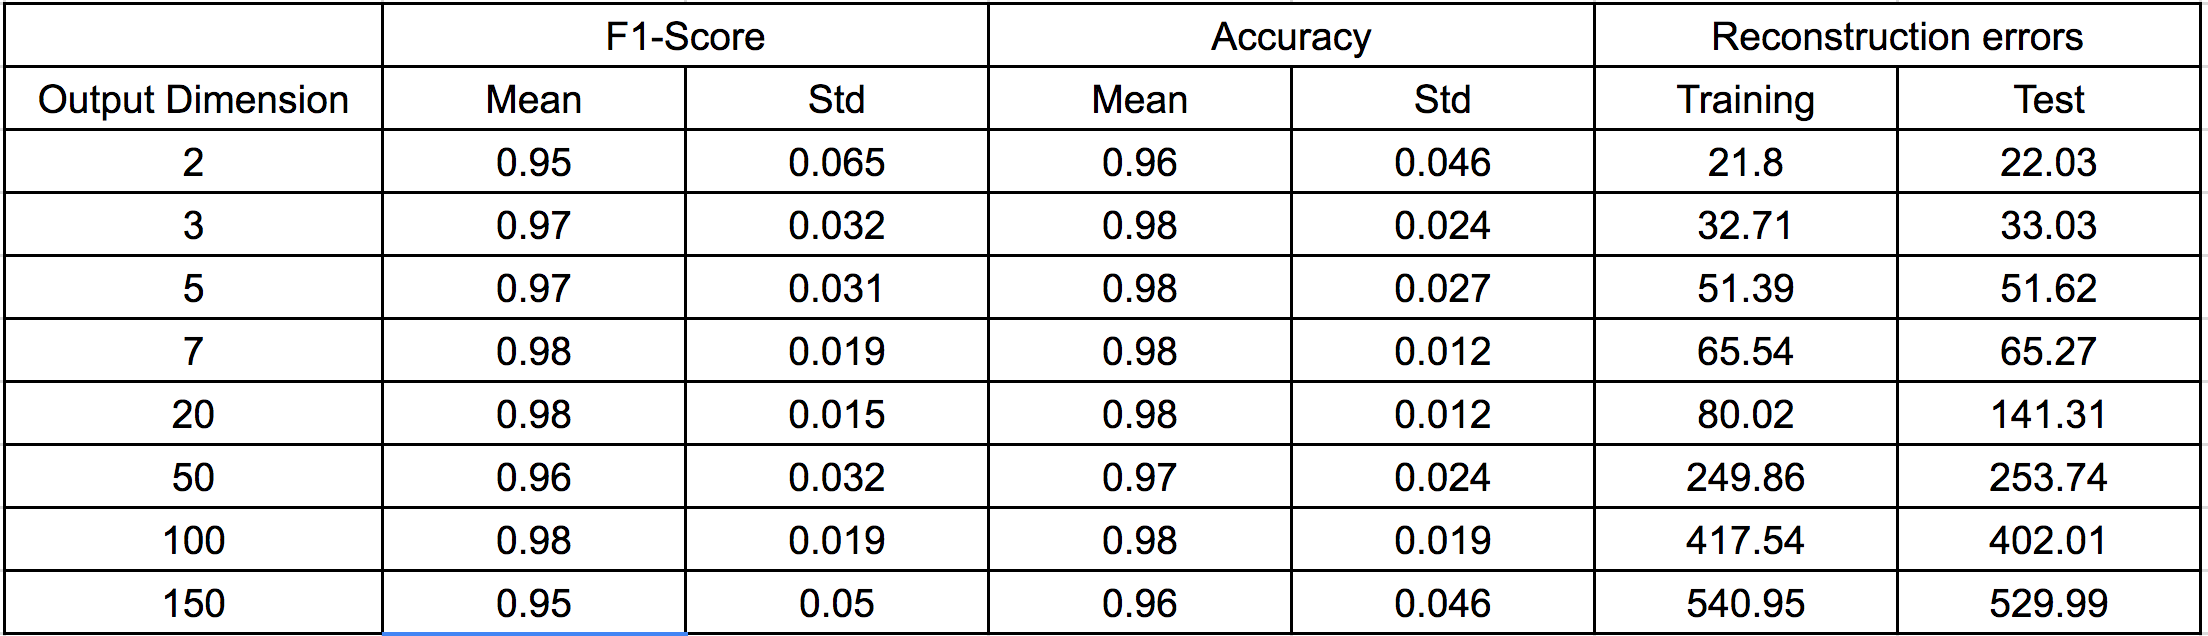
\includegraphics[scale=0.35]{thesis/images/LCGC_output_dimension_results.png}
    \caption{Results of LCGC under different number of output dimensions}
    \label{fig:lcpc_results_C}
\end{figure}
We generated the dataset by mixing two latent  Gaussian processes. For every sample $s \in S$, we mixed either two gaussian processes or one linear and one gaussian process with 40 percent probability. S scaled samples are then generated  by keeping mixing matrix constant throughout the samples. The labels are assigned according to the mixing, i.e. +1 when one of the process has a positive linear slope and  -1 otherwise.

\subsubsection{Effect of output dimensions}
To test the impact of output dimensions, we keep number of latent processes constant (P=2) but change mixing matrix corresponding to a different number of output dimensions. 

Fig \ref{fig:lcpc_results_C} shows our model’s performance with the artificial dataset for different values of C. It’s easy to see that model's performance remain pretty stable even when number of output dimension is near or more than the number of samples. Since model projects data back to a much tighter latent and removes much of redundant columns due to prior on mixing matrix favoring smaller values, number of output dimensions end up losing it's relevance, giving pretty much stable performance over increased number of output dimensions.
\subsubsection{Number of samples}
\begin{figure}
    \centering
    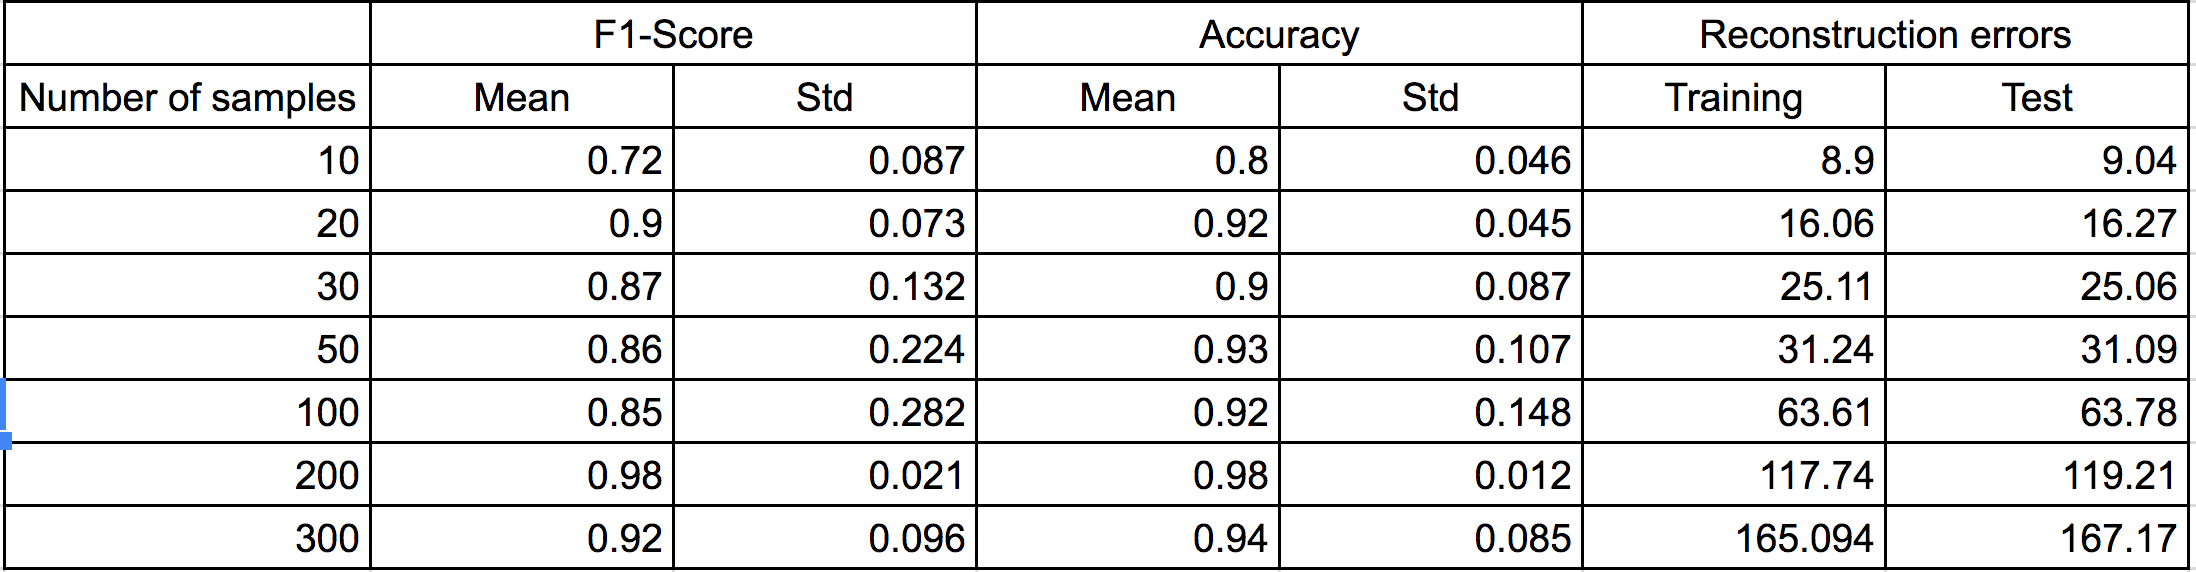
\includegraphics[scale=0.35]{thesis/images/LCGC_samples_results.png}
    \caption{Results of LCGC with varying number of samples in output}
    \label{fig:lcpc_results_samples}
\end{figure}

Fig \ref{fig:lcpc_results_samples} shows us the results when sampling resolution is varied for fixed number of output dimensions (C=3 in this example). Once again we see that model is robust with in a large range of sampling resolution. Even 20 percent of maximum possible samples are enough to yield good enough f1 Scores. Predictive power of course increases as the number of samples available to the model becomes higher.

\subsubsection{Inducing points}
Finally, we also tested classification power of model with different number of inducing points, The ability to use lesser number of inducing points with minimum impact on performance makes the model scalable since sparse solution drastically reduces the time complexity of inference procedure from $O(N^3)$ to $O(Nn^3)$, where $n << N$. 
As evident from the Fig \ref{fig:lcpc_results_induction}, even 50 percent reduction in the number of points is able to achieve good enough classification accuracy on the dataset indicating that huge speed ups are possible with  presented sparse solution of the model.

\begin{figure}
    \centering
    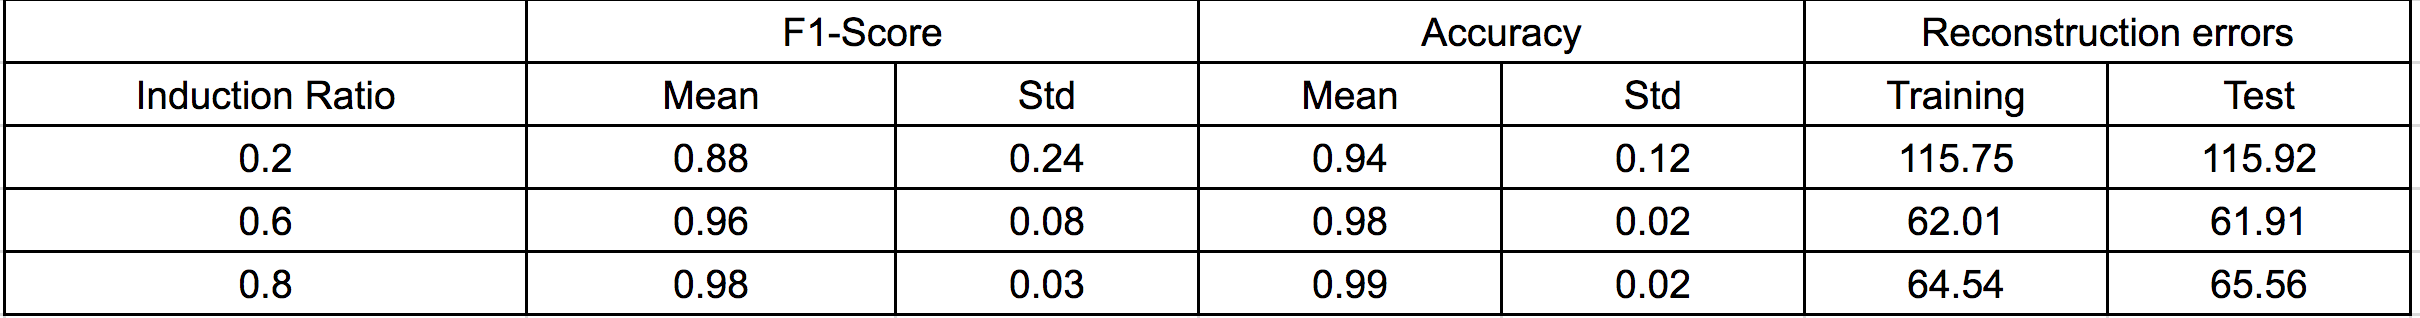
\includegraphics[scale=0.35]{thesis/images/LCGC_inducing_results.png}
    \caption{Results of LCGC under different levels of induction ratio}
    \label{fig:lcpc_results_induction}
\end{figure}
\subsection{Synthetic control dataset}
We use a benchmark dataset namely ‘synthetic control data set’ [1] from UCI to test the classification performance of our  model and then comparing it against other standard classification models. The dataset has a collection of 600 series instances with five different trends: Upward and downward trend, upward and downward shift, cyclic trend and random noise. For the experiment we divide entire datset into training and test instances and try  to predict the correct classification for test data using the parameters learned during training. 
\begin{figure}
    \centering
    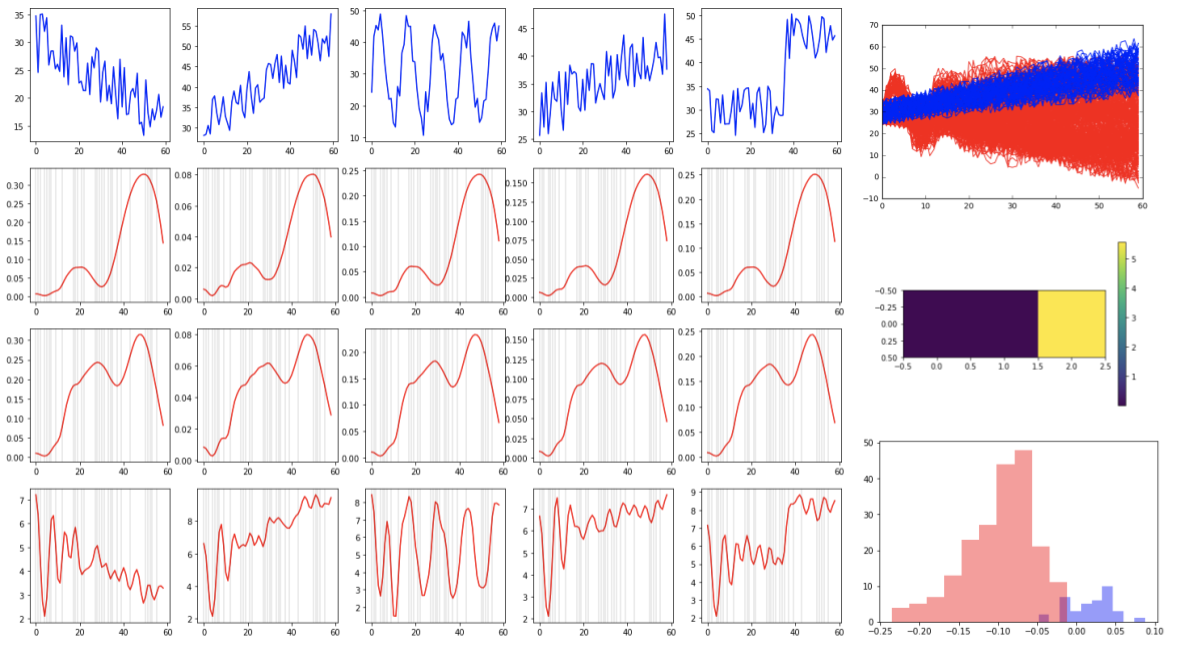
\includegraphics[scale=0.35]{thesis/images/LCGC_real_classification.png}
    \caption{LCGC results on synthetic control dataset: Left: Top rows shows the samples from test dataset, Bottom three rows show respective guessed latent processes. Right top: training dataset with blue showing postive instances, middle: Infered mixing matrix, bottom: Separation inferred among test instances.}
    \label{fig:lcgc_classifications}
\end{figure}
For this experiment, LCGC model was employed with it's default settings (P=3, gaussian Kernels) and 0.8 induction ratio. Top right side of the Figure displays the training dataset with positive classes colored in blue. Rest of the figure shows the result of classification;  mixing matrix in top middle and the guessed latent processes (2-4th row)for few samples of test instances (first row) in the bottom. Top right shows the clear separation between most of the latent values $l*$ of test instances. As we can observe guesses latent processes of LCGC accurately mimic the actual instance thereby decently separating the test instances into their respective classes. 

Moreover, Figure \ref{fig:lcpc_classification_results} shows the comparison between LDA, logistic regression and linear SVM with LCMGP, and we can see that even with 0.8 induction ratio and only default settings performance of LCGC is at par with other time tested algorithms. All of the other classification models were taken from publicly available Scipy implementations[2].
\subsection{Conclusion}
\begin{figure}
    \centering
    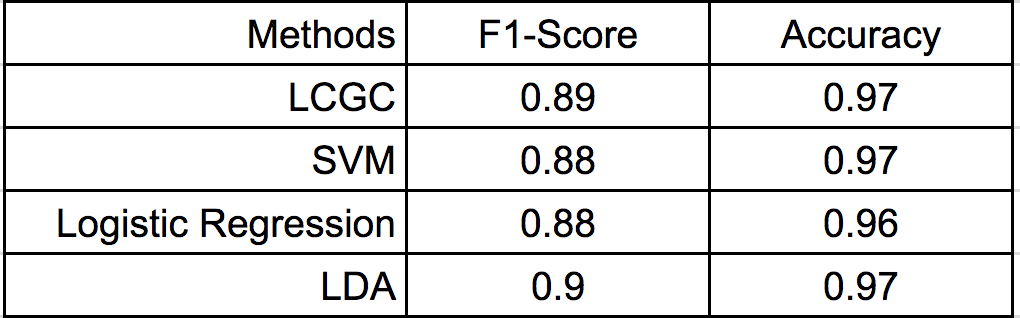
\includegraphics[scale=0.45]{thesis/images/LCGC_classification_results.png}
    \caption{Comparative results of different classification methods on synthetic control dataset }
    \label{fig:lcpc_classification_results}
\end{figure}

Results on artificially generated dataset were promising and indicate that the model's result will be stable under varrying conditions. The results of classification experiment with synthetic control dataset are onpar with the other state of the art classification algorthms, specially considering that a very simple implementation of LCGC was used, optimizations for hyper parmaters as well as inducing point selecition schemes can be used to improve the predictive power of model. The only caveat during experimentation is due to the variational nature of model a specially bad initialization of parameters might stop model from converging within specified number of iterations. These events are however rare and overall results of all of our experiments indicate that LCGC can be a promising model in cases  where the data is generated through a long series of multiple measurements for example in medical, meteorological settings etc.
